\documentclass{standalone}
\usepackage{tikz}
\usepackage{nono}
\begin{document}
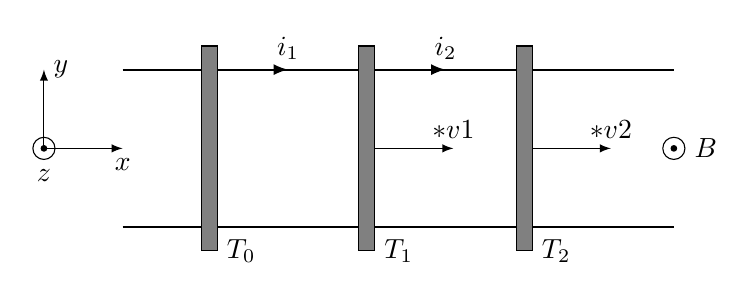
\begin{tikzpicture} 
  \draw[thick] (0, 0) -- (7, 0);
  \draw[thick] (0, 2) -- (7, 2);
  \draw[fill=gray] (1, -0.3) node[right=0.2cm] {$T_0$}  rectangle (1.2, 2.3);
  \draw[fill=gray] (3, -0.3) node[right=0.2cm] {$T_1$}  rectangle (3.2, 2.3);
  \draw[fill=gray] (5, -0.3) node[right=0.2cm] {$T_2$}  rectangle (5.2, 2.3);
  \draw (7, 1) circle(4pt) node[right=4pt]{$\vv{B}$};
  \draw[fill] (7, 1) circle(1pt);
  \draw[thick, -latex] (2, 2) -- ++(0.1, 0) node[above]{$i_1$}; 
  \draw[thick, -latex] (4, 2) -- ++(0.1, 0) node[above]{$i_2$}; 
  \draw[-latex] (3.2, 1) -- ++(1, 0) node[above]{$\vv*{v}{1}$}; 
  \draw[-latex] (5.2, 1) -- ++(1, 0) node[above]{$\vv*{v}{2}$}; 
  \draw[-latex] (-1, 1) coordinate(O) -- ++(1,0) node[below]{$x$}; 
  \draw[-latex] (O) coordinate(O) -- ++(0,1) node[right]{$y$}; 
  \draw (O) circle(4pt) node[below=4pt]{$z$}; 
  \draw[fill] (O) circle(1pt); 
\end{tikzpicture}
\end{document}
